\documentclass[11pt, a4paper]{article}

% Fonts and Encoding
\usepackage[utf8]{inputenc}
\usepackage[T1]{fontenc}

% Math and Symbols
\usepackage{amsmath, amssymb, amsthm, amsfonts, mathrsfs, mathtools}

% Layout and Geometry
\usepackage{geometry}
\geometry{a4paper, margin=1in}

% Formatting and Graphics
\usepackage{graphicx, xcolor, enumitem, booktabs, array, tabularx}

% TikZ for Illustrations
\usepackage{tikz}
\usetikzlibrary{arrows.meta, positioning, shapes.geometric, calc, backgrounds, matrix}

% Clickable Links and TOC
\usepackage{hyperref}
\hypersetup{
    colorlinks=true,
    linkcolor=blue,
    filecolor=magenta,      
    urlcolor=cyan,
    pdftitle={Advanced Mathematics: Multivariate Expectations},
}

% Theorem Environments
\newtheorem{theorem}{Theorem}[section]
\newtheorem{lemma}[theorem]{Lemma}
\newtheorem{proposition}[theorem]{Proposition}
\newtheorem{corollary}[theorem]{Corollary}
\theoremstyle{definition}
\newtheorem{definition}{Definition}[section]
\newtheorem{axiom}{Axiom}[section]
\newtheorem{example}{Example}[section]
\theoremstyle{remark}
\newtheorem{remark}{Remark}[section]

% Custom Commands (Enforced standard notation)
\newcommand{\R}{\mathbb{R}}
\newcommand{\N}{\mathbb{N}}
\newcommand{\Z}{\mathbb{Z}}
\newcommand{\Q}{\mathbb{Q}}
\newcommand{\E}{\mathbb{E}}
\newcommand{\Prob}{\mathbb{P}}
\newcommand{\F}{\mathcal{F}}
\newcommand{\Var}{\mathrm{Var}}
\newcommand{\Cov}{\mathrm{Cov}}

\title{\textbf{Advanced Abstract Mathematics: \\ Expected Values of Multivariate Distributions}}
\author{Tashfeen Omran}
\date{\today}

\begin{document}

\maketitle
\tableofcontents
\newpage

\section{Comprehensive Introduction, Context, and Prerequisites}

\subsection{Core Concepts \& Axioms}
In the rigorous study of probability theory, we operate within a formal probability space $(\Omega, \F, \Prob)$, where $\Omega$ is the sample space, $\F$ is a $\sigma$-algebra of measurable events, and $\Prob$ is a probability measure. A random variable $Y$ is defined as an $\F$-measurable function mapping $\Omega$ to the real numbers $\R$. 

When extending this to multivariate distributions, we consider random vectors, such as $(Y_1, Y_2)$, mapping $\Omega \to \R^2$. The expected value (or expectation) of a function of these random variables, $g(Y_1, Y_2)$, is formally defined via the Lebesgue integral with respect to the joint probability measure:
\[
\E[g(Y_1, Y_2)] = \int_{\Omega} g(Y_1(\omega), Y_2(\omega)) \, d\Prob(\omega)
\]
In applied contexts, this abstract integral reduces to a Riemann integral over the joint probability density function (pdf) $f(y_1, y_2)$ for continuous variables, or a double summation over the joint probability mass function (pmf) $p(y_1, y_2)$ for discrete variables.

\subsection{Intuition and Set-Theoretic Foundations}
Intuitively, the expected value represents the center of mass of a distribution. When we apply a transformation $g(Y_1, Y_2)$, we are mapping the original space $\R^2$ into a new space $\R$. The Law of the Unconscious Statistician (LOTUS) guarantees that we do not need to find the complex derived distribution of $Z = g(Y_1, Y_2)$ to compute its expectation; we can integrate directly over the original partition of $\R^2$ weighted by the original measure.

\subsection{Historical Context and Motivation}
The formalization of multivariate expectations was driven by the need to model interacting systems in physics (e.g., statistical mechanics) and early biometric studies by Francis Galton and Karl Pearson. The foundational crisis of probability—where geometric probabilities led to paradoxes like Bertrand's Paradox—forced Andrey Kolmogorov in 1933 to ground probability in measure theory. This ensured that operations like the expectation of sums and products were logically consistent and free from contradiction.

\subsection{Key Theorems, Lemmas, and Formulas}
The following theorems form the bedrock of linear operations on random variables:
\begin{theorem}[Expectation of a Constant]
Let $c \in \R$ be a constant. Then $\E[c] = c$.
\end{theorem}
\begin{theorem}[Homogeneity of Expectation]
Let $g(Y_1, Y_2)$ be a measurable function and $c \in \R$. Then $\E[c g(Y_1, Y_2)] = c \E[g(Y_1, Y_2)]$.
\end{theorem}
\begin{theorem}[Linearity of Expectation]
For measurable functions $g_1, \dots, g_k$, 
\[
\E\left[\sum_{i=1}^k g_i(Y_1, Y_2)\right] = \sum_{i=1}^k \E[g_i(Y_1, Y_2)]
\]
\end{theorem}
\begin{theorem}[Product of Independent Variables]
If $Y_1$ and $Y_2$ are independent random variables, and $g, h$ are measurable functions, then
\[
\E[g(Y_1)h(Y_2)] = \E[g(Y_1)]\E[h(Y_2)]
\]
provided the expectations exist.
\end{theorem}

\subsection{Prerequisites}
Mastery of this chapter requires:
\begin{itemize}
    \item \textbf{Multivariable Calculus:} Proficiency in setting up and evaluating double integrals, particularly over non-rectangular domains.
    \item \textbf{Set Theory:} Understanding partitions, intersections, and unions of events.
    \item \textbf{Basic Probability:} Familiarity with univariate distributions (Binomial, Geometric, Exponential, Gamma, Normal, Chi-Square).
\end{itemize}

\newpage
\section{Detailed Homework Solutions}

\subsection{Problem 5.72}
\textbf{Statement:} The joint distribution of $Y_1$ and $Y_2$ is given by a table. The marginal of $Y_1$ is Binomial with $n=2, p=1/3$. Find (a) $\E[Y_1]$, (b) $\Var(Y_1)$, (c) $\E[Y_1 - Y_2]$.

\textbf{Proof/Solution:}
\begin{enumerate}[label=\alph*)]
    \item \textbf{Direct Computation:} Since $Y_1 \sim \text{Bin}(2, 1/3)$, we use the standard formula for the expectation of a binomial distribution:
    \[
    \E[Y_1] = np = 2 \left(\frac{1}{3}\right) = \frac{2}{3}
    \]
    \item \textbf{Variance Computation:} The variance of a binomial distribution is $np(1-p)$:
    \[
    \Var(Y_1) = np(1-p) = 2 \left(\frac{1}{3}\right) \left(\frac{2}{3}\right) = \frac{4}{9}
    \]
    \item \textbf{Linearity of Expectation:} We need $\E[Y_1 - Y_2] = \E[Y_1] - \E[Y_2]$. First, we find the marginal distribution of $Y_2$ by summing the columns of the provided joint probability table:
    \begin{align*}
        \Prob(Y_2 = 0) &= \frac{1}{9} + \frac{2}{9} + \frac{1}{9} = \frac{4}{9} \\
        \Prob(Y_2 = 1) &= \frac{2}{9} + \frac{2}{9} + 0 = \frac{4}{9} \\
        \Prob(Y_2 = 2) &= \frac{1}{9} + 0 + 0 = \frac{1}{9}
    \end{align*}
    Now, compute $\E[Y_2]$:
    \[
    \E[Y_2] = \sum_{y_2=0}^2 y_2 \Prob(Y_2 = y_2) = 0\left(\frac{4}{9}\right) + 1\left(\frac{4}{9}\right) + 2\left(\frac{1}{9}\right) = \frac{6}{9} = \frac{2}{3}
    \]
    By Linearity of Expectation:
    \[
    \E[Y_1 - Y_2] = \E[Y_1] - \E[Y_2] = \frac{2}{3} - \frac{2}{3} = 0
    \]
\end{enumerate}
\hfill $\blacksquare$

\subsection{Problem 5.73}
\textbf{Statement:} The joint pmf is $p(y_1, y_2) = \frac{\binom{4}{y_1}\binom{3}{y_2}\binom{2}{3-y_1-y_2}}{\binom{9}{3}}$. Find the expected number of married executives ($Y_1$) among the three selected.

\textbf{Proof/Solution:}
This represents a multivariate hypergeometric distribution. We are selecting $n=3$ individuals from a total population of $N=9$. The population contains $K=4$ married executives. 
To find $\E[Y_1]$, we only need the marginal distribution of $Y_1$. By the definition of the multivariate hypergeometric distribution, the marginal distribution of any single component is a standard univariate hypergeometric distribution.
Thus, $Y_1 \sim \text{Hypergeometric}(N=9, K=4, n=3)$.
The expectation of a hypergeometric random variable is given by $n \frac{K}{N}$:
\[
\E[Y_1] = 3 \left(\frac{4}{9}\right) = \frac{12}{9} = \frac{4}{3}
\]
\hfill $\blacksquare$

\subsection{Problem 5.74}
\textbf{Statement:} $f(y_1, y_2) = 1$ for $0 \leq y_1 \leq 1, 0 \leq y_2 \leq 1$. Find (a) $\E[Y_1 - Y_2]$, (b) $\E[Y_1 Y_2]$, (c) $\E[Y_1^2 + Y_2^2]$, (d) $\Var(Y_1 Y_2)$.

\textbf{Proof/Solution:}
The joint density factors as $f(y_1, y_2) = 1 \cdot 1 = f_1(y_1)f_2(y_2)$. Thus, $Y_1$ and $Y_2$ are independent Uniform$(0,1)$ random variables. We know $\E[Y_i] = 1/2$ and $\E[Y_i^2] = \int_0^1 y^2 dy = 1/3$.
\begin{enumerate}[label=\alph*)]
    \item $\E[Y_1 - Y_2] = \E[Y_1] - \E[Y_2] = \frac{1}{2} - \frac{1}{2} = 0$.
    \item By independence (Theorem 5.9): $\E[Y_1 Y_2] = \E[Y_1]\E[Y_2] = \left(\frac{1}{2}\right)\left(\frac{1}{2}\right) = \frac{1}{4}$.
    \item By linearity: $\E[Y_1^2 + Y_2^2] = \E[Y_1^2] + \E[Y_2^2] = \frac{1}{3} + \frac{1}{3} = \frac{2}{3}$.
    \item To find $\Var(Y_1 Y_2)$, we use $\Var(W) = \E[W^2] - (\E[W])^2$ where $W = Y_1 Y_2$.
    \[
    \E[(Y_1 Y_2)^2] = \E[Y_1^2 Y_2^2] = \E[Y_1^2]\E[Y_2^2] = \left(\frac{1}{3}\right)\left(\frac{1}{3}\right) = \frac{1}{9}
    \]
    \[
    \Var(Y_1 Y_2) = \frac{1}{9} - \left(\frac{1}{4}\right)^2 = \frac{1}{9} - \frac{1}{16} = \frac{16 - 9}{144} = \frac{7}{144}
    \]
\end{enumerate}
\hfill $\blacksquare$

\subsection{Problem 5.75}
\textbf{Statement:} $f(y_1, y_2) = e^{-(y_1+y_2)}$ for $y_1 > 0, y_2 > 0$. Find various expectations and probabilities.

\textbf{Proof/Solution:}
The density factors as $e^{-y_1} e^{-y_2}$, meaning $Y_1$ and $Y_2$ are independent Exponential random variables with $\lambda = 1$. Thus, $\E[Y_i] = 1$ and $\Var(Y_i) = 1$.
\begin{enumerate}[label=\alph*)]
    \item $\E[Y_1 + Y_2] = \E[Y_1] + \E[Y_2] = 1 + 1 = 2$. \\ \relax
    Since they are independent, $\Var(Y_1 + Y_2) = \Var(Y_1) + \Var(Y_2) = 1 + 1 = 2$.
    \item $\Prob(Y_1 - Y_2 > 3) = \Prob(Y_1 > Y_2 + 3)$. We set up the double integral:
    \begin{align*}
        \Prob(Y_1 > Y_2 + 3) &= \int_0^\infty \int_{y_2+3}^\infty e^{-y_1} e^{-y_2} \, dy_1 \, dy_2 \\
        &= \int_0^\infty e^{-y_2} \left[ -e^{-y_1} \right]_{y_2+3}^\infty \, dy_2 \\
        &= \int_0^\infty e^{-y_2} e^{-(y_2+3)} \, dy_2 = e^{-3} \int_0^\infty e^{-2y_2} \, dy_2 \\
        &= e^{-3} \left[ -\frac{1}{2} e^{-2y_2} \right]_0^\infty = \frac{1}{2} e^{-3}
    \end{align*}
    \item By symmetry of the i.i.d. distributions, $\Prob(Y_1 - Y_2 < -3) = \Prob(Y_2 - Y_1 > 3) = \frac{1}{2} e^{-3}$.
    \item $\E[Y_1 - Y_2] = \E[Y_1] - \E[Y_2] = 1 - 1 = 0$. \\ \relax
    $\Var(Y_1 - Y_2) = \Var(Y_1) + \Var(-Y_2) = \Var(Y_1) + (-1)^2\Var(Y_2) = 1 + 1 = 2$.
    \item We notice that $\Var(Y_1 + Y_2) = \Var(Y_1 - Y_2) = 2$. This occurs because the covariance is zero (due to independence), eliminating the cross-term in the variance expansion.
\end{enumerate}
\hfill $\blacksquare$

\subsection{Problem 5.76}
\textbf{Statement:} $f(y_1, y_2) = 4y_1 y_2$ for $0 \leq y_1 \leq 1, 0 \leq y_2 \leq 1$. Find (a) $\E[Y_1]$, (b) $\Var(Y_1)$, (c) $\E[Y_1 - Y_2]$.

\textbf{Proof/Solution:}
The variables are independent since $f(y_1, y_2) = (2y_1)(2y_2)$. The marginal is $f_1(y_1) = 2y_1$ for $y_1 \in [0,1]$.
\begin{enumerate}[label=\alph*)]
    \item $\E[Y_1] = \int_0^1 y_1 (2y_1) \, dy_1 = \int_0^1 2y_1^2 \, dy_1 = \left[ \frac{2}{3}y_1^3 \right]_0^1 = \frac{2}{3}$.
    \item $\E[Y_1^2] = \int_0^1 y_1^2 (2y_1) \, dy_1 = \int_0^1 2y_1^3 \, dy_1 = \left[ \frac{1}{2}y_1^4 \right]_0^1 = \frac{1}{2}$. \\ \relax
    $\Var(Y_1) = \E[Y_1^2] - (\E[Y_1])^2 = \frac{1}{2} - \left(\frac{2}{3}\right)^2 = \frac{1}{2} - \frac{4}{9} = \frac{9 - 8}{18} = \frac{1}{18}$.
    \item By symmetry, $\E[Y_2] = 2/3$. Thus, $\E[Y_1 - Y_2] = \frac{2}{3} - \frac{2}{3} = 0$.
\end{enumerate}
\hfill $\blacksquare$

\subsection{Problem 5.77}
\textbf{Statement:} $f(y_1, y_2) = 6(1 - y_2)$ for $0 \leq y_1 \leq y_2 \leq 1$. Find expectations and variances.

\textbf{Proof/Solution:}
First, we find the marginal densities.
For $Y_2$:
\[
f_2(y_2) = \int_0^{y_2} 6(1 - y_2) \, dy_1 = 6(1 - y_2)[y_1]_0^{y_2} = 6y_2(1 - y_2), \quad 0 \leq y_2 \leq 1
\]
This is a Beta distribution with $\alpha=2, \beta=2$.
For $Y_1$:
\[
f_1(y_1) = \int_{y_1}^1 6(1 - y_2) \, dy_2 = 6 \left[ y_2 - \frac{y_2^2}{2} \right]_{y_1}^1 = 6 \left( \frac{1}{2} - y_1 + \frac{y_1^2}{2} \right) = 3(1 - y_1)^2, \quad 0 \leq y_1 \leq 1
\]
This is a Beta distribution with $\alpha=1, \beta=3$.
\begin{enumerate}[label=\alph*)]
    \item $\E[Y_1] = \int_0^1 3y_1(1-y_1)^2 \, dy_1 = 3 \int_0^1 (y_1 - 2y_1^2 + y_1^3) \, dy_1 = 3\left(\frac{1}{2} - \frac{2}{3} + \frac{1}{4}\right) = 3\left(\frac{1}{12}\right) = \frac{1}{4}$. \\ \relax
    $\E[Y_2] = \int_0^1 6y_2^2(1-y_2) \, dy_2 = 6\left(\frac{1}{3} - \frac{1}{4}\right) = 6\left(\frac{1}{12}\right) = \frac{1}{2}$.
    \item $\E[Y_1^2] = \int_0^1 3y_1^2(1-y_1)^2 \, dy_1 = 3\left(\frac{1}{3} - \frac{2}{4} + \frac{1}{5}\right) = 3\left(\frac{1}{30}\right) = \frac{1}{10}$. \\ \relax
    $\Var(Y_1) = \frac{1}{10} - \left(\frac{1}{4}\right)^2 = \frac{1}{10} - \frac{1}{16} = \frac{8 - 5}{80} = \frac{3}{80}$. \\ \relax
    $\E[Y_2^2] = \int_0^1 6y_2^3(1-y_2) \, dy_2 = 6\left(\frac{1}{4} - \frac{1}{5}\right) = \frac{6}{20} = \frac{3}{10}$. \\ \relax
    $\Var(Y_2) = \frac{3}{10} - \left(\frac{1}{2}\right)^2 = \frac{3}{10} - \frac{1}{4} = \frac{6 - 5}{20} = \frac{1}{20}$.
    \item $\E[Y_1 - 3Y_2] = \E[Y_1] - 3\E[Y_2] = \frac{1}{4} - 3\left(\frac{1}{2}\right) = \frac{1}{4} - \frac{6}{4} = -\frac{5}{4}$.
\end{enumerate}
\hfill $\blacksquare$

\subsection{Problem 5.78}
\textbf{Statement:} $f(y_1, y_2) = 1$ for $0 \leq y_1 \leq 2, 0 \leq y_2 \leq 1, 2y_2 \leq y_1$. Find expectations, variances, and limits for $Y_1 - Y_2$.

\textbf{Proof/Solution:}
The domain is a triangle with vertices $(0,0), (2,0), (2,1)$.
Marginal for $Y_1$:
\[
f_1(y_1) = \int_0^{y_1/2} 1 \, dy_2 = \frac{y_1}{2}, \quad 0 \leq y_1 \leq 2
\]
Marginal for $Y_2$:
\[
f_2(y_2) = \int_{2y_2}^2 1 \, dy_1 = 2 - 2y_2, \quad 0 \leq y_2 \leq 1
\]
\begin{enumerate}[label=\alph*)]
    \item $\E[Y_1] = \int_0^2 y_1 \left(\frac{y_1}{2}\right) \, dy_1 = \left[ \frac{y_1^3}{6} \right]_0^2 = \frac{8}{6} = \frac{4}{3}$. \\ \relax
    $\E[Y_2] = \int_0^1 y_2 (2 - 2y_2) \, dy_2 = \left[ y_2^2 - \frac{2y_2^3}{3} \right]_0^1 = 1 - \frac{2}{3} = \frac{1}{3}$.
    \item $\E[Y_1^2] = \int_0^2 \frac{y_1^3}{2} \, dy_1 = \left[ \frac{y_1^4}{8} \right]_0^2 = 2$. \\ \relax
    $\Var(Y_1) = 2 - \left(\frac{4}{3}\right)^2 = 2 - \frac{16}{9} = \frac{2}{9}$. \\ \relax
    $\E[Y_2^2] = \int_0^1 (2y_2^2 - 2y_2^3) \, dy_2 = \frac{2}{3} - \frac{2}{4} = \frac{1}{6}$. \\ \relax
    $\Var(Y_2) = \frac{1}{6} - \left(\frac{1}{3}\right)^2 = \frac{1}{6} - \frac{1}{9} = \frac{1}{18}$.
    \item $\E[Y_1 - Y_2] = \E[Y_1] - \E[Y_2] = \frac{4}{3} - \frac{1}{3} = 1$.
    \item To find $\Var(Y_1 - Y_2)$, we need $\Cov(Y_1, Y_2) = \E[Y_1 Y_2] - \E[Y_1]\E[Y_2]$.
    \begin{align*}
        \E[Y_1 Y_2] &= \int_0^1 \int_{2y_2}^2 y_1 y_2 \, dy_1 \, dy_2 = \int_0^1 y_2 \left[ \frac{y_1^2}{2} \right]_{2y_2}^2 \, dy_2 \\
        &= \int_0^1 y_2 (2 - 2y_2^2) \, dy_2 = \int_0^1 (2y_2 - 2y_2^3) \, dy_2 = 1 - \frac{2}{4} = \frac{1}{2}
    \end{align*}
    $\Cov(Y_1, Y_2) = \frac{1}{2} - \left(\frac{4}{3}\right)\left(\frac{1}{3}\right) = \frac{1}{2} - \frac{4}{9} = \frac{1}{18}$. \\ \relax
    $\Var(Y_1 - Y_2) = \Var(Y_1) + \Var(Y_2) - 2\Cov(Y_1, Y_2) = \frac{2}{9} + \frac{1}{18} - 2\left(\frac{1}{18}\right) = \frac{4}{18} + \frac{1}{18} - \frac{2}{18} = \frac{3}{18} = \frac{1}{6}$. \\ \relax
    \textbf{Limits:} The minimum of $Y_1 - Y_2$ occurs on the boundary $y_1 = 2y_2$, yielding $2y_2 - y_2 = y_2 \geq 0$. The maximum occurs at $(2,0)$, yielding $2 - 0 = 2$. Thus, $Y_1 - Y_2 \in [0, 2]$.
\end{enumerate}
\hfill $\blacksquare$

\subsection{Problem 5.79}
\textbf{Statement:} $Y_1, Y_2$ are uniformly distributed over the triangle with vertices $(-1,0), (1,0), (0,1)$. Find $\E[Y_1 Y_2]$.

\textbf{Proof/Solution:}
The area of the triangle is $\frac{1}{2}(2)(1) = 1$. Thus, $f(y_1, y_2) = 1$ over the region.
The region is symmetric with respect to the $y_2$-axis (i.e., invariant under $y_1 \to -y_1$).
The function $g(y_1, y_2) = y_1 y_2$ is an odd function with respect to $y_1$.
Therefore, the integral over the symmetric domain is exactly zero:
\[
\E[Y_1 Y_2] = \iint_{\text{Triangle}} y_1 y_2 \, dy_1 \, dy_2 = 0
\]
\hfill $\blacksquare$

\subsection{Problem 5.80}
\textbf{Statement:} $f(y_1, y_2) = y_1 + y_2$ for $0 \leq y_1 \leq 1, 0 \leq y_2 \leq 1$. Find $\E[30Y_1 + 25Y_2]$.

\textbf{Proof/Solution:}
First, find $\E[Y_1]$:
\begin{align*}
    \E[Y_1] &= \int_0^1 \int_0^1 y_1(y_1 + y_2) \, dy_2 \, dy_1 = \int_0^1 \left[ y_1^2 y_2 + \frac{y_1 y_2^2}{2} \right]_{y_2=0}^1 \, dy_1 \\
    &= \int_0^1 \left( y_1^2 + \frac{y_1}{2} \right) \, dy_1 = \left[ \frac{y_1^3}{3} + \frac{y_1^2}{4} \right]_0^1 = \frac{1}{3} + \frac{1}{4} = \frac{7}{12}
\end{align*}
By symmetry of the joint density, $\E[Y_2] = \frac{7}{12}$.
Using linearity of expectation:
\[
\E[30Y_1 + 25Y_2] = 30\E[Y_1] + 25\E[Y_2] = 55 \left(\frac{7}{12}\right) = \frac{385}{12} \approx 32.083
\]
\hfill $\blacksquare$

\subsection{Problem 5.81}
\textbf{Statement:} $f(y_1, y_2) = \frac{1}{8} y_1 e^{-(y_1+y_2)/2}$ for $y_1 > 0, y_2 > 0$. Find $\E[Y_2 / Y_1]$.

\textbf{Proof/Solution:}
The joint density factors into $f(y_1, y_2) = \left( \frac{1}{4} y_1 e^{-y_1/2} \right) \left( \frac{1}{2} e^{-y_2/2} \right)$.
Thus, $Y_1$ and $Y_2$ are independent. $Y_1 \sim \text{Gamma}(\alpha=2, \beta=2)$ and $Y_2 \sim \text{Exponential}(\beta=2)$.
By independence, $\E\left[\frac{Y_2}{Y_1}\right] = \E[Y_2] \E[Y_1^{-1}]$.
We know $\E[Y_2] = \beta = 2$.
For $Y_1^{-1}$:
\[
\E[Y_1^{-1}] = \int_0^\infty y_1^{-1} \left( \frac{1}{4} y_1 e^{-y_1/2} \right) \, dy_1 = \frac{1}{4} \int_0^\infty e^{-y_1/2} \, dy_1 = \frac{1}{4} (2) = \frac{1}{2}
\]
Therefore, $\E\left[\frac{Y_2}{Y_1}\right] = 2 \left(\frac{1}{2}\right) = 1$.
\hfill $\blacksquare$

\subsection{Problem 5.82}
\textbf{Statement:} $f(y_1, y_2) = 1/y_1$ for $0 \leq y_2 \leq y_1 \leq 1$. Find $\E[Y_1 - Y_2]$.

\textbf{Proof/Solution:}
\begin{align*}
    \E[Y_1] &= \int_0^1 \int_0^{y_1} y_1 \left(\frac{1}{y_1}\right) \, dy_2 \, dy_1 = \int_0^1 \int_0^{y_1} 1 \, dy_2 \, dy_1 = \int_0^1 y_1 \, dy_1 = \frac{1}{2} \\
    \E[Y_2] &= \int_0^1 \int_0^{y_1} y_2 \left(\frac{1}{y_1}\right) \, dy_2 \, dy_1 = \int_0^1 \frac{1}{y_1} \left[ \frac{y_2^2}{2} \right]_0^{y_1} \, dy_1 = \int_0^1 \frac{y_1}{2} \, dy_1 = \frac{1}{4}
\end{align*}
Thus, $\E[Y_1 - Y_2] = \frac{1}{2} - \frac{1}{4} = \frac{1}{4}$.
\hfill $\blacksquare$

\subsection{Problem 5.83}
\textbf{Statement:} $p(y) = (1/2)^{y+1}$ for $y = 0, 1, 2, \dots$. Find $\E[Y]$.

\textbf{Proof/Solution:}
This is a Geometric distribution modeling the number of failures before the first success, with $p = 1/2$.
\[
\E[Y] = \sum_{y=0}^\infty y \left(\frac{1}{2}\right)^{y+1} = \frac{1}{2} \sum_{y=1}^\infty y \left(\frac{1}{2}\right)^y
\]
Using the standard series identity $\sum_{k=1}^\infty k x^k = \frac{x}{(1-x)^2}$ for $|x| < 1$:
\[
\E[Y] = \frac{1}{2} \left( \frac{1/2}{(1 - 1/2)^2} \right) = \frac{1}{2} \left( \frac{1/2}{1/4} \right) = \frac{1}{2} (2) = 1
\]
\hfill $\blacksquare$

\subsection{Problem 5.84}
\textbf{Statement:} $Y_1, Y_2$ are independent Geometric random variables with parameter $p$. Find expectations and variances related to $Y_1 - Y_2$.

\textbf{Proof/Solution:}
For a standard Geometric distribution (number of trials until first success), $\E[Y_i] = \frac{1}{p}$ and $\Var(Y_i) = \frac{1-p}{p^2} = \frac{q}{p^2}$.
\begin{enumerate}[label=\alph*)]
    \item $\E[Y_1] = \frac{1}{p}$, $\E[Y_2] = \frac{1}{p}$, $\E[Y_1 - Y_2] = 0$.
    \item $\E[Y_1^2] = \Var(Y_1) + (\E[Y_1])^2 = \frac{q}{p^2} + \frac{1}{p^2} = \frac{q+1}{p^2} = \frac{2-p}{p^2}$. \\ \relax
    Similarly, $\E[Y_2^2] = \frac{2-p}{p^2}$. \\ \relax
    By independence, $\E[Y_1 Y_2] = \E[Y_1]\E[Y_2] = \frac{1}{p^2}$.
    \item $\E[(Y_1 - Y_2)^2] = \E[Y_1^2 - 2Y_1 Y_2 + Y_2^2] = \frac{2-p}{p^2} - \frac{2}{p^2} + \frac{2-p}{p^2} = \frac{4 - 2p - 2}{p^2} = \frac{2(1-p)}{p^2} = \frac{2q}{p^2}$. \\ \relax
    Since $\E[Y_1 - Y_2] = 0$, $\Var(Y_1 - Y_2) = \E[(Y_1 - Y_2)^2] = \frac{2q}{p^2}$.
    \item Using Chebyshev's Inequality: $\Prob(|Y_1 - Y_2 - \mu| < k\sigma) \geq 1 - \frac{1}{k^2}$. \\ \relax
    We want probability at least $8/9$, so $1 - \frac{1}{k^2} = \frac{8}{9} \implies k^2 = 9 \implies k = 3$. \\ \relax
    The interval is $\mu \pm 3\sigma = 0 \pm 3\sqrt{\frac{2q}{p^2}} = \left( -\frac{3\sqrt{2q}}{p}, \frac{3\sqrt{2q}}{p} \right)$.
\end{enumerate}
\hfill $\blacksquare$

\subsection{Problem 5.85}
\textbf{Statement:} $f(y_1, y_2) = [1 - \alpha(1 - 2e^{-y_1})(1 - 2e^{-y_2})]e^{-y_1-y_2}$ for $y_1, y_2 \geq 0$. Marginals are Exponential(1). Find expectations and variances.

\textbf{Proof/Solution:}
\begin{enumerate}[label=\alph*)]
    \item Since marginals are Exp(1), $\E[Y_1] = 1$ and $\E[Y_2] = 1$.
    \item $\Var(Y_1) = 1$ and $\Var(Y_2) = 1$.
    \item (Implied c) $\E[Y_1 - Y_2] = 1 - 1 = 0$.
    \item (Implied d) To find $\E[Y_1 Y_2]$, we integrate:
    \[
    \E[Y_1 Y_2] = \int_0^\infty \int_0^\infty y_1 y_2 \left[ e^{-y_1-y_2} - \alpha(e^{-y_1} - 2e^{-2y_1})(e^{-y_2} - 2e^{-2y_2}) \right] dy_1 dy_2
    \]
    This splits into $\E[Y_1]\E[Y_2] - \alpha I_1 I_2$, where $I_1 = \int_0^\infty y_1(e^{-y_1} - 2e^{-2y_1}) dy_1$.
    \[
    I_1 = \int_0^\infty y_1 e^{-y_1} dy_1 - 2 \int_0^\infty y_1 e^{-2y_1} dy_1 = 1 - 2\left(\frac{1}{4}\right) = \frac{1}{2}
    \]
    Thus, $\E[Y_1 Y_2] = (1)(1) - \alpha\left(\frac{1}{2}\right)\left(\frac{1}{2}\right) = 1 - \frac{\alpha}{4}$.
    \item (Implied e) $\Var(Y_1 - Y_2) = \Var(Y_1) + \Var(Y_2) - 2\Cov(Y_1, Y_2)$. \\ \relax
    $\Cov(Y_1, Y_2) = \E[Y_1 Y_2] - \E[Y_1]\E[Y_2] = \left(1 - \frac{\alpha}{4}\right) - 1 = -\frac{\alpha}{4}$. \\ \relax
    $\Var(Y_1 - Y_2) = 1 + 1 - 2\left(-\frac{\alpha}{4}\right) = 2 + \frac{\alpha}{2}$.
\end{enumerate}
\hfill $\blacksquare$

\subsection{Problem 5.86}
\textbf{Statement:} $Z \sim N(0,1)$, $Y_1 \sim \chi^2_{\nu_1}$, $Y_2 \sim \chi^2_{\nu_2}$, all independent. Find expectations and variances of $W = Z/\sqrt{Y_1}$ and $U = Y_1/Y_2$.

\textbf{Proof/Solution:}
\begin{enumerate}[label=\alph*)]
    \item $W = Z Y_1^{-1/2}$. By independence, $\E[W] = \E[Z]\E[Y_1^{-1/2}] = 0 \cdot \E[Y_1^{-1/2}] = 0$. \\ \relax
    This requires $\E[Y_1^{-1/2}]$ to exist, which holds for $\nu_1 > 1$. \\ \relax
    $\Var(W) = \E[W^2] - 0 = \E[Z^2]\E[Y_1^{-1}]$. We know $\E[Z^2] = 1$. \\ \relax
    For a $\chi^2_\nu$ variable, $\E[Y^{-1}] = \frac{1}{\nu - 2}$ for $\nu > 2$. \\ \relax
    Thus, $\Var(W) = 1 \cdot \frac{1}{\nu_1 - 2} = \frac{1}{\nu_1 - 2}$. Assumption: $\nu_1 > 2$.
    \item $U = Y_1 Y_2^{-1}$. By independence, $\E[U] = \E[Y_1]\E[Y_2^{-1}] = \nu_1 \left( \frac{1}{\nu_2 - 2} \right) = \frac{\nu_1}{\nu_2 - 2}$. Assumption: $\nu_2 > 2$. \\ \relax
    $\Var(U) = \E[U^2] - (\E[U])^2 = \E[Y_1^2]\E[Y_2^{-2}] - \frac{\nu_1^2}{(\nu_2 - 2)^2}$. \\ \relax
    $\E[Y_1^2] = \Var(Y_1) + (\E[Y_1])^2 = 2\nu_1 + \nu_1^2 = \nu_1(\nu_1 + 2)$. \\ \relax
    $\E[Y_2^{-2}] = \frac{1}{(\nu_2 - 2)(\nu_2 - 4)}$ for $\nu_2 > 4$. \\ \relax
    $\Var(U) = \frac{\nu_1(\nu_1 + 2)}{(\nu_2 - 2)(\nu_2 - 4)} - \frac{\nu_1^2}{(\nu_2 - 2)^2}$. Assumption: $\nu_2 > 4$.
\end{enumerate}
\hfill $\blacksquare$

\subsection{Problem 5.87}
\textbf{Statement:} $Y_1, Y_2$ are independent $\chi^2$ with $\nu_1, \nu_2$ degrees of freedom. Find $\E[Y_1 + Y_2]$ and $\Var(Y_1 + Y_2)$.

\textbf{Proof/Solution:}
For $Y_i \sim \chi^2_{\nu_i}$, $\E[Y_i] = \nu_i$ and $\Var(Y_i) = 2\nu_i$.
\begin{enumerate}[label=\alph*)]
    \item By linearity: $\E[Y_1 + Y_2] = \E[Y_1] + \E[Y_2] = \nu_1 + \nu_2$.
    \item By independence: $\Var(Y_1 + Y_2) = \Var(Y_1) + \Var(Y_2) = 2\nu_1 + 2\nu_2 = 2(\nu_1 + \nu_2)$.
\end{enumerate}
\hfill $\blacksquare$

\subsection{Problem 5.88}
\textbf{Statement:} Expected number of tosses to observe all 6 faces of a die (Coupon Collector's Problem).

\textbf{Proof/Solution:}
Let $Y$ be the total number of tosses. We can write $Y = \sum_{i=1}^6 Y_i$, where $Y_i$ is the number of additional tosses required to get the $i$-th distinct face after $i-1$ distinct faces have been observed.
Each $Y_i$ follows a Geometric distribution with success probability $p_i = \frac{7-i}{6}$.
The expectation of a Geometric random variable is $1/p_i$.
\begin{align*}
    \E[Y] &= \sum_{i=1}^6 \E[Y_i] = \sum_{i=1}^6 \frac{6}{7-i} = 6 \left( \frac{1}{6} + \frac{1}{5} + \frac{1}{4} + \frac{1}{3} + \frac{1}{2} + 1 \right) \\
    &= 6 \left( \frac{10 + 12 + 15 + 20 + 30 + 60}{60} \right) = 6 \left( \frac{147}{60} \right) = \frac{147}{10} = 14.7
\end{align*}
\hfill $\blacksquare$

\newpage
\section{In-Depth Analysis of Problems and Techniques}

\subsection{Problem Types and Logical Strategies}
\begin{itemize}
    \item \textbf{Marginalization \& Linearity (e.g., 5.72, 5.77, 5.78):} The core strategy is to avoid computing the complex distribution of $Y_1 - Y_2$. Instead, we integrate out one variable to find the marginal densities $f_1(y_1)$ and $f_2(y_2)$, compute their individual expectations, and apply $\E[Y_1 - Y_2] = \E[Y_1] - \E[Y_2]$.
    \item \textbf{Independence Exploitation (e.g., 5.74, 5.75, 5.81, 5.86):} When the joint density factors as $f(y_1, y_2) = g(y_1)h(y_2)$, the variables are independent. The strategy shifts to using $\E[g(Y_1)h(Y_2)] = \E[g(Y_1)]\E[h(Y_2)]$. This is especially powerful for ratios, transforming $\E[Y_1/Y_2]$ into $\E[Y_1]\E[Y_2^{-1}]$.
    \item \textbf{Symmetry Arguments (e.g., 5.79):} Recognizing that a domain is symmetric and the integrand is an odd function allows us to deduce that the integral is zero without performing tedious calculus.
\end{itemize}

\subsection{Key Analytical and Logical Manipulations}
\begin{itemize}
    \item \textbf{The Variance Expansion Trick:} To find $\Var(Y_1 - Y_2)$, we expand it as $\Var(Y_1) + \Var(Y_2) - 2\Cov(Y_1, Y_2)$. If independent, the covariance term vanishes.
    \item \textbf{Geometric Series Manipulation:} In Problem 5.83, evaluating the expectation of a discrete distribution required the analytical trick of differentiating the geometric series: $\sum k x^k = x/(1-x)^2$.
    \item \textbf{Gamma Function Integration:} In Problem 5.81, recognizing the kernel of a Gamma distribution allowed us to evaluate $\int y^{-1} e^{-y/2} dy$ instantly without integration by parts.
\end{itemize}

\newpage
\section{"Cheatsheet", Visuals, and Tips for Success}

\subsection{Theorems \& Equivalences}
\renewcommand{\arraystretch}{1.5}
\noindent
\begin{tabularx}{\textwidth}{>{\raggedright\arraybackslash}p{4cm} >{$\displaystyle}X<{$}}
\toprule
\textbf{Concept} & \textbf{Mathematical Formulation} \\
\midrule
Linearity of Expectation & \E[aX + bY] = a\E[X] + b\E[Y] \\
\addlinespace[4pt]
Independence Product & \E[XY] = \E[X]\E[Y] \quad \text{(if } X, Y \text{ independent)} \\
\addlinespace[4pt]
Covariance Definition & \Cov(X, Y) = \E[XY] - \E[X]\E[Y] \\
\addlinespace[4pt]
Variance of a Sum & \Var(aX \pm bY) = a^2\Var(X) + b^2\Var(Y) \pm 2ab\Cov(X, Y) \\
\bottomrule
\end{tabularx}

\subsection{Set \& Logic Illustrations}
The following TikZ diagram illustrates the integration region from Problem 5.78, demonstrating how the bounds of the joint density dictate the limits of integration for marginalization.

\vspace{1em}
\begin{center}
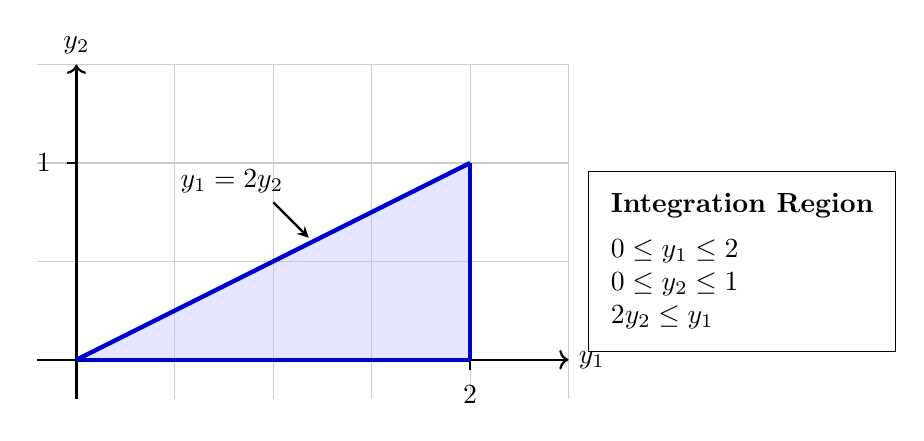
\begin{tikzpicture}[scale=2.5]
    % 1) Fill background
    \fill[blue!10] (0,0) -- (2,0) -- (2,1) -- cycle;
    
    % 2) Grid and Axes
    \draw[thin, gray!40, step=0.5] (-0.2,-0.2) grid (2.5, 1.5);
    \draw[->, thick] (-0.2,0) -- (2.5,0) node[right] {$y_1$};
    \draw[->, thick] (0,-0.2) -- (0,1.5) node[above] {$y_2$};
    
    % 3) Primary plots
    \draw[ultra thick, blue!80!black] (0,0) -- (2,1);
    \draw[ultra thick, blue!80!black] (2,0) -- (2,1);
    \draw[ultra thick, blue!80!black] (0,0) -- (2,0);
    
    % Microscopic tick marks
    \draw[thick] (2,0) -- (2,-0.05) node[below=2pt] {$2$};
    \draw[thick] (0,1) -- (-0.05,1) node[left=2pt] {$1$};
    
    % Callout arrow
    \draw[->, >=stealth, shorten >=2pt, thick] (1, 0.8) -- (1.2, 0.6);
    \node[above left] at (1.1, 0.8) {$y_1 = 2y_2$};
    
    % 4) Nodes and Labels (Single Node Multiline Rule)
    \node[align=left, anchor=west, inner sep=8pt, draw, fill=white] at (2.6, 0.5) {
        \textbf{Integration Region} \\[4pt]
        $\displaystyle 0 \leq y_1 \leq 2$ \\
        $\displaystyle 0 \leq y_2 \leq 1$ \\
        $\displaystyle 2y_2 \leq y_1$
    };
\end{tikzpicture}
\end{center}

\subsection{Heuristics \& "Cheats"}
\begin{itemize}
    \item \textbf{The "Zero Covariance" Trap:} If $X$ and $Y$ are independent, $\Cov(X,Y) = 0$. However, the converse is \textit{false}. If $\Cov(X,Y) = 0$, they might still be dependent (e.g., $X \sim U(-1,1)$ and $Y = X^2$).
    \item \textbf{Ratio Shortcut:} Never assume $\E[X/Y] = \E[X]/\E[Y]$. You must use $\E[X \cdot Y^{-1}]$, and if independent, it becomes $\E[X]\E[Y^{-1}]$.
\end{itemize}

\newpage
\section{Conceptual Synthesis and The "Big Picture"}

\subsection{Thematic Connections}
The central theme of this chapter is the \textit{preservation of linear structure} under the expectation operator. Because expectation is fundamentally a Lebesgue integral, it inherits the linearity of integration. This allows us to decompose complex, high-dimensional random systems into manageable, one-dimensional components. 

\subsection{Forward and Backward Links}
\begin{itemize}
    \item \textbf{Backward Links:} This topic builds directly on univariate integration and the axioms of probability spaces. It extends the 1D Law of the Unconscious Statistician to $\R^n$.
    \item \textbf{Forward Links:} Understanding multivariate expectations and covariance is the absolute prerequisite for defining Conditional Expectation $\E[X|Y]$, which is a random variable itself. This, in turn, forms the foundation of Martingale theory and Stochastic Calculus (e.g., Ito Integrals).
\end{itemize}

\section{Abstract Real-World Modeling (AI, ML, \& Quant Finance)}

\subsection{Concrete Scenarios}
\begin{enumerate}
    \item \textbf{Quantitative Finance (Portfolio Variance):} In Modern Portfolio Theory (Markowitz), the expected return of a portfolio is a linear combination of individual asset returns. However, the risk (variance) depends heavily on the covariance matrix of the assets.
    \item \textbf{Machine Learning (Bayesian Neural Networks):} In variational inference, we often need to compute the expected value of the log-likelihood over a posterior distribution of weights, requiring high-dimensional multivariate expectations.
\end{enumerate}

\subsection{Model Problem Setup: Risk-Neutral Pricing of a Basket Option}
Consider a financial market with two correlated assets, $S_1(t)$ and $S_2(t)$, modeled by a 2D Geometric Brownian Motion under the risk-neutral measure $\mathbb{Q}$:
\begin{align*}
    dS_1(t) &= r S_1(t) dt + \sigma_1 S_1(t) dW_1(t) \\
    dS_2(t) &= r S_2(t) dt + \sigma_2 S_2(t) dW_2(t)
\end{align*}
where $dW_1 dW_2 = \rho dt$. A European basket call option with strike $K$ pays out $g(S_1(T), S_2(T)) = \max(w_1 S_1(T) + w_2 S_2(T) - K, 0)$ at maturity $T$.
The fundamental theorem of asset pricing states the price $V_0$ is the discounted expected value:
\[
V_0 = e^{-rT} \E^{\mathbb{Q}} \left[ \max(w_1 S_1(T) + w_2 S_2(T) - K, 0) \right]
\]
Because the payoff function is non-linear (due to the $\max$ operator), we cannot simply pass the expectation inside. We must evaluate the 2D integral over the joint log-normal density of $(S_1(T), S_2(T))$, which relies entirely on the multivariate expectation theorems established in this chapter.

\newpage
\section{Common Variations and Untested Concepts}

A critical concept often tested in advanced courses but missing from this specific homework set is the \textbf{Law of Total Expectation} (The Tower Property).

\textbf{Theorem:} For random variables $X$ and $Y$, $\E[X] = \E[\E[X|Y]]$.

\textbf{Worked Example:} Let $N \sim \text{Poisson}(\lambda)$ be the number of customers entering a store. Let $X_i \sim \text{Exponential}(\mu)$ be the amount of money spent by the $i$-th customer. Find the expected total revenue $R = \sum_{i=1}^N X_i$.

\textit{Proof:} We condition on $N$:
\[
\E[R | N = n] = \E\left[ \sum_{i=1}^n X_i \right] = \sum_{i=1}^n \E[X_i] = n\mu
\]
Thus, the random variable $\E[R|N]$ is equal to $N\mu$.
By the Law of Total Expectation:
\[
\E[R] = \E[\E[R|N]] = \E[N\mu] = \mu\E[N] = \mu\lambda
\]
\hfill $\blacksquare$

\section{Advanced Diagnostic Testing: "Find the Flaw"}

Below are five proofs containing a subtle logical or mathematical flaw. Act as the grader to find the error.

\subsection{Flawed Proof 1}
\textbf{Claim:} If $X \sim U(0,1)$ and $Y \sim U(0,1)$ are independent, then $\E[X/Y] = 1$. \\ \relax
\textit{Proof:} By linearity and independence, $\E[X/Y] = \E[X] / \E[Y]$. Since $X$ and $Y$ have the same distribution, $\E[X] = 1/2$ and $\E[Y] = 1/2$. Therefore, $(1/2)/(1/2) = 1$.

\subsection{Flawed Proof 2}
\textbf{Claim:} If $\E[XY] = \E[X]\E[Y]$, then $X$ and $Y$ are independent. \\ \relax
\textit{Proof:} The definition of independence states that the joint distribution factors. If the expectation of the product factors into the product of expectations, the underlying integrals must have factored, proving independence.

\subsection{Flawed Proof 3}
\textbf{Claim:} For $f(x,y) = 2$ on $0 \leq x \leq y \leq 1$, $\E[X] = 1/2$. \\ \relax
\textit{Proof:} $\E[X] = \int_0^1 \int_0^1 x (2) \, dx \, dy = \int_0^1 [x^2]_0^1 \, dy = \int_0^1 1 \, dy = 1$. Wait, the domain is a triangle, so $\E[X] = 1/2 \times 1 = 1/2$.

\subsection{Flawed Proof 4}
\textbf{Claim:} $\Var(X - Y) = \Var(X) - \Var(Y)$ for independent variables. \\ \relax
\textit{Proof:} Variance is a linear operator for independent variables. Therefore, $\Var(aX + bY) = a\Var(X) + b\Var(Y)$. Letting $a=1, b=-1$, we get $\Var(X - Y) = \Var(X) - \Var(Y)$.

\subsection{Flawed Proof 5}
\textbf{Claim:} If $X \sim \text{Cauchy}(0,1)$, then $\E[X] = 0$. \\ \relax
\textit{Proof:} The density $f(x) = \frac{1}{\pi(1+x^2)}$ is symmetric around 0. The integral $\int_{-\infty}^\infty \frac{x}{\pi(1+x^2)} dx$ evaluates to 0 because the integrand is an odd function.

\vspace{2em}
\hrule
\vspace{1em}
\subsection*{Solution Key (Grader's Resolution)}
\textbf{Flaw 1:} The expectation operator is linear, but it does not distribute over division. $\E[X/Y] = \E[X]\E[Y^{-1}]$. For $Y \sim U(0,1)$, $\E[Y^{-1}] = \int_0^1 y^{-1} dy = \infty$. The expectation is undefined. \\ \relax
\textbf{Flaw 2:} $\E[XY] = \E[X]\E[Y]$ only implies zero covariance (uncorrelated), not independence. Example: $X \sim U(-1,1)$ and $Y = X^2$. \\ \relax
\textbf{Flaw 3:} The limits of integration were ignored in the first step, and a geometric heuristic was improperly applied. The correct integral is $\int_0^1 \int_0^y 2x \, dx \, dy = \int_0^1 y^2 \, dy = 1/3$. \\ \relax
\textbf{Flaw 4:} Variance scales by the square of the constant. $\Var(bY) = b^2\Var(Y)$. Thus, for $b=-1$, $\Var(-Y) = (-1)^2\Var(Y) = \Var(Y)$. The correct formula is $\Var(X) + \Var(Y)$. \\ \relax
\textbf{Flaw 5:} The Lebesgue integral $\int |x| f(x) dx$ must be finite for the expectation to exist. For the Cauchy distribution, $\int_0^\infty \frac{x}{\pi(1+x^2)} dx = \infty$. Thus, the expectation is undefined, not zero.

\end{document}